\chapter{Analisis Masalah dan Perancangan Solusi}
Pada bab ini diuraikan analisis persoalan \textit{Performance Regression Analysis} yang telah diuraikan pada Bab I. Hasil dari bab ini digunakan untuk merancang kakas yang akan diimplementasikan seperti yang akan dijelaskan pada Bab IV. 


\section{Analisis Masalah}
\label{analisis-masalah}

Seiring dengan meningkatnya kompleksitas dari aplikasi Microservice, seperti dengan meningkatnya jumlah service dan keterhubungan antar service yang ada di dalamnya, akan meningkat juga kompleksitas untuk melakukan \textit{monitoring} terhadap kinerja pada keseluruhan aplikasi Microservice. Salah satu isu penting terkait dengan kinerja adalah regresi atau penurunan terhadap kinerja. Kebutuhan untuk dengan segera menentukan penyebab utama dari regresi pada sistem menjadi penting apabila regresi terjadi pada lingkungan produksi yang langsung melayani \textit{request} dari pelanggan, sehingga apabila tidak diatasi dengan segera akan berdampak langsung terhadap pengalaman pengguna dalam menggunakan aplikasi. 

Terdapat dua pendekatan yang dapat dilakukan untuk mengatasi permasalahan regresi kinerja \citep{regression-detection}, yaitu:
\begin{enumerate}
	\item Deteksi regresi dilakukan setelah aplikasi selesai dikembangkan dan di-\textit{deploy} pada lingkungan terdedikasi
	\item Deteksi regresi dilakukan sebelum aplikasi selesai dikembangkan dan di-\textit{deploy} dan melakukan studi terhadap perubahan yang dihasilkan pada \textit{source code}
\end{enumerate}  

Mengingat sifat dari Microservice yang terdistribusi, akan menjadi sulit bagi \textit{developer} jika pendeteksian regresi dilakukan dengan pendekatan individual pada masing-masing service yang ada terlebih ketika jumlah service yang ada sudah sangat banyak dan hubungan interdependensi antar service menjadi rumit. Oleh karena itu, untuk mengatasi regresi kinerja pada aplikasi berbasis Microservice, dibutuhkanlah pendekatan yang tidak mengharuskan \textit{developer} untuk melakukan pencarian sumber masalah pada masing-masing service secara individu. Sehingga pada kasus deteksi dan analisis regresi kinerja aplikasi berbasis Microservice, pendekatan pertama lebih cocok untuk digunakan.

Salah satu teknologi yang dapat digunakan untuk melakukan \textit{monitoring} dan analisis regresi pada sebuah sistem terdistribusi seperti Microservice adalah \textit{distributed tracing}. Dengan bantuan mekanisme \textit{span} dari \textit{trace}, metrik-metrik kinerja dalam aplikasi berbasis Microservice dapat dilacak secara menyeluruh. Dalam kasus penggunaan seperti yang telah disebutkan sebelumnya, \textit{distributed tracing} cocok untuk digunakan dalam melakukan analisis regresi kinerja atau \textit{Performance Regression Analysis} dalam sebuah aplikasi berbasis Microservice sebab \textit{developer} tidak perlu menganalisis satu per satu \textit{service} yang ada terutama setelah \textit{service} sudah di-\textit{deploy}.

Oleh karena itu, dapat dirumuskan alur kerja yang harus dilakukan oleh sistem \textit{Performance Regression Analysis} (PRA) sebagai berikut:
\begin{enumerate}
	\item Sistem harus dapat mendeteksi ketika terjadi regresi pada aplikasi berbasis Microservice
	\item Sistem harus dapat menentukan sumber atau akar permasalahan dari regresi setelah terdeteksi
\end{enumerate}

Sudah terdapat beberapa pendekatan yang dapat digunakan untuk melakukan analisis regresi seperti yang ada pada subbab \ref{ch2-algo}. Melihat kebutuhan dari sistem PRA di atas, dari beberapa pendekatan yang ada pada subbab tersebut, penulis menilai ada dua pendekatan yang dapat digunakan yaitu pendekatan Analisis Kumulatif pada \ref{approach-cumulative} dan pendekatan Analisis Agregasi dan Korelasi pada \ref{approach-corr}. Analisis Kumulatif dapat digunakan untuk menentukan apakah telah terjadi regresi pada aplikasi dengan melakukan perbandingan antara CDF \textit{baseline} dengan CDF dari aplikasi yang sedang berjalan. Ketika didapatkan dari hasil tes statistik K-S bahwa kedua sampel data merupakan dua distribusi yang berbeda, mengindikasikan bahwa telah terjadi regresi atau penyimpangan dari kinerja seharusnya, sistem PRA selanjutnya akan melakukan analisis akar permasalahan dengan metode Analisis Agregasi dan Korelasi untuk mendapatkan penyebab dari regresi melalui analisis \textit{crtical path}.

Gambar \ref{alur-pra} menggambarkan fase yang akan dilakukan oleh sistem PRA. Secara umum, akan terdapat dua fase yang akan dilakukan yaitu fase \textit{baseline loading phase} dan fase \textit{realtime analysis phase}. Fase pertama yaitu \textit{loading phase} akan mencari data dari aktivitas aplikasi yang bersifat stabil yang dapat digunakan sebagai \textit{baseline} atau acuan bagi analisis yang akan dilakukan pada tahap-tahap selanjutnya. Fase ini akan menghasilkan dua buah artifak yaitu data \textit{latency} dari semua trace yang direkam oleh sistem \textit{tracing}, dan data operasi yang terjadi pada \textit{critical path} semua \textit{trace} beserta nilai \textit{latency}-nya yang akan disimpan juga sebagai pasangan \textit{key-value}. 

Fase berikutnya adalah fase analisis secara \textit{realtime}. Ada beberapa tahap analisis yang akan dilakukan pada fase ini.  Tahap analisis pertama akan membandingkan hasil transformasi CDF histogram \textit{tracing} yang sedang berlangsung secara \textit{realtime} dengan CDF \textit{baseline} hasil fase \textit{loading}. Perbandingan tersebut akan dilakukan dalam periode tertentu. Perbandingan dari kedua CDF tadi akan menghasilkan statistik Kolmogorov-Smirnov (K-S). Jika statistik K-S yang dihasilkan melebihi batas \textit{threshold} \textit{significance level} dari statistik K-S, maka dapat disimpulkan bahwa terjadi regresi pada periode \textit{capture} histogram tersebut. 

Jika terdeteksi terjadi regresi, tahap selanjutnya adalah melakukan analisis korelasi seperti yang telah dijelaskan pada \ref{approach-corr}. Sampel perbandingan \textit{trace} yang akan digunakan adalah sampel \textit{trace} yang berasal dari data sampel \textit{baseline}. Hasil korelasi kemudian diurutkan dan akan dicek selanjutnya mana saja fitur seperti \textit{service} yang nilai koefisien korelasinya melebihi \textit{threshold} batas korelasi. Kemudian selanjutnya akan dihitung nilai kontribusi \textit{critical path} pada \textit{service} yang terindikasi mengalami regresi dan hasil perhitungan kontribusi \textit{latency} dari \textit{critical path} tersebut akan dibandingkan dengan data \textit{latency} \textit{critical path} yang berasal dari perhitungan \textit{baseline}. Dari perbandingan tadi, akan diurutkan dan didapatlah hasil operasi mana yang memiliki perubahan \textit{latency} terbesar dan menjadi kandidat kuat sebagai akar permasalahan penyebab regresi.

\begin{figure}[!htb]
	\centering
	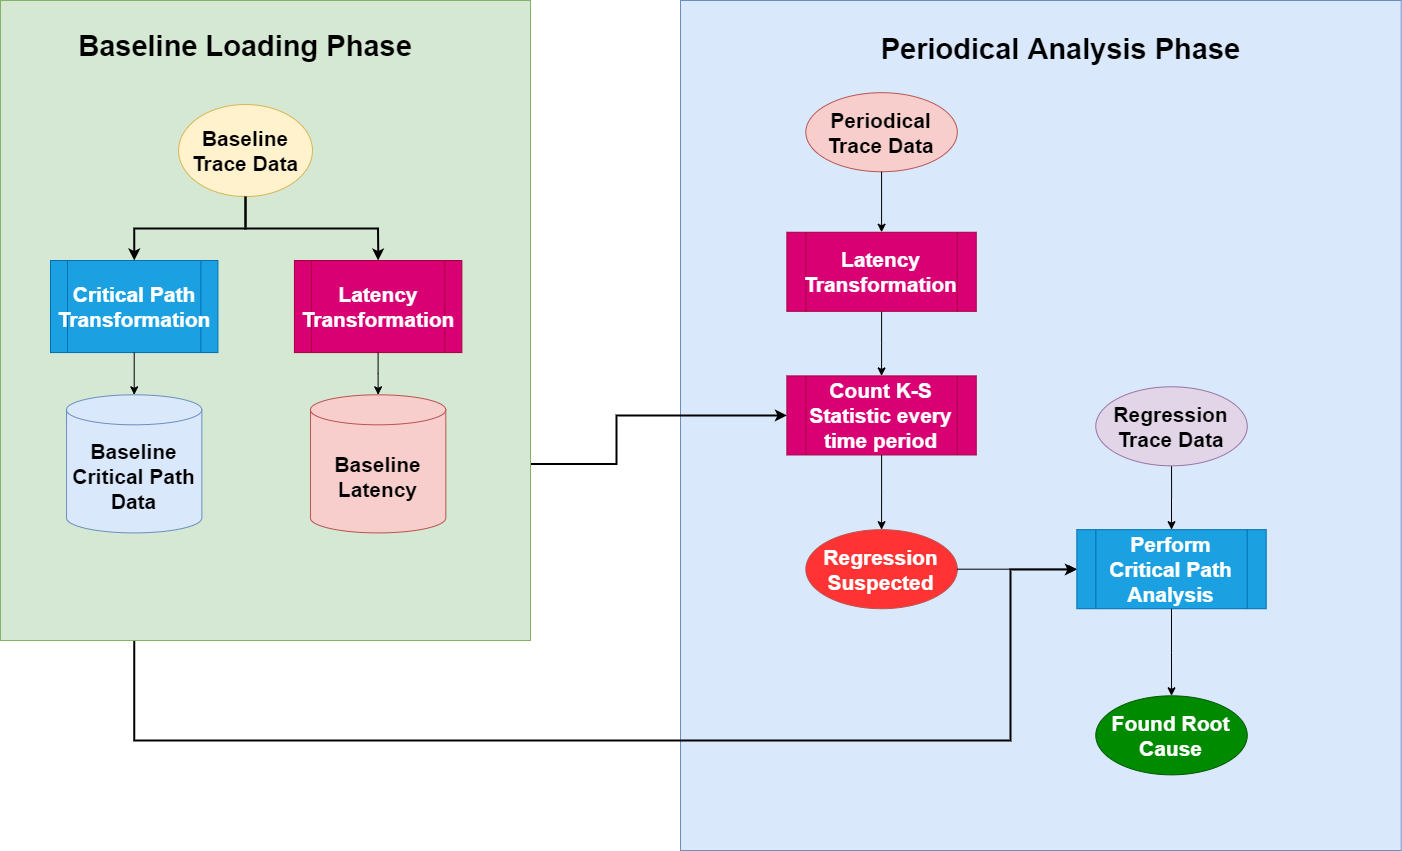
\includegraphics[width=1\textwidth,scale=1.5]{resources/ch3/alur_v2.png}
	\caption{Alur sistem \textit{Performance Regression Analysis}}
	\label{alur-pra}
\end{figure}

\section{Rancangan Solusi}

\subsection{Pemilihan Solusi \textit{tracing}}

Dari pemaparan alur sistem \textit{Performance Regression Analysis} pada subbab \ref{analisis-masalah}, dapat dirumuskan beberapa kriteria sistem \textit{distributed tracing} yang akan digunakan. Daftar kriteria dapat dilihat pada Tabel \ref{ch3-trace-crit}.

Dari berbagai jenis solusi \textit{distributed tracing} yang sudah ada seperti pada subbab \ref{terkait}, penulis menilai Zipkin merupakan solusi yang tepat untuk digunakan sebab memenuhi semua kriteria pada tabel di atas. Untuk kriteria TC-1, Zipkin menggunakan metode instrumentasi secara \textit{active} dengan menambahkan informasi header \textit{span} induk dan \textit{span} anak pada setiap \textit{request} sehingga hubungan kausalitas antar \textit{service} dalam \textit{request} dapat dicatat sebagai hubungan induk-anak dalam \textit{span}. Untuk kriteria TC-2, sudah terdapat dukungan untuk membuat \textit{deployment} di Kubernetes dari komunitas \textit{Open Source} \citep{zipkin-ambassador}. Untuk kriteria TC-3, Zipkin menyediakan dukungan ekstensi bagi komponen \textit{collector} dan \textit{storage} dari pihak ketiga dan sudah didukung secara \textit{native} untuk beberapa komponen \citep{zipkin-storage}.

\begin{small}
	\begin{longtable}{ | p{3cm} | p{10cm} |}
		\caption{Kriteria pemilihan solusi \textit{tracing}}
		\label{ch3-trace-crit}                                                           
		\\ \hline
		\centering\bfseries{ID Kriteria} & \centering\bfseries{Deskripsi} \tabularnewline \hline
		\endfirsthead
		TC-1 & Komponen instrumentasi dapat menyediakan informasi kausalitas antar \textit{service} yang terjadi selama \textit{request} pada \textit{span} \\ \hline
		TC-2 & Komponen \textit{deployment} menyediakan dukungan untuk Kubernetes \\ \hline
		TC-3 & Komponen \textit{deplyoment} menyediakan dukungan untuk \textit{storage} eksternal \\ \hline
	\end{longtable}
\end{small}

\subsection{Arsitektur Solusi}

Gambar \ref{arch-pra} menunjukkan arsitektur dari solusi \textit{distributed tracing} yang akan digunakan untuk melakukan \textit{Performance Regression Analysis}. Komponen utama \textit{tracing} yang akan digunakan sesuai dengan arsitektur \textit{tracing} yang dimiliki oleh Zipkin seperti pada gambar \ref{zipkin-arch}. Komponen instrumentasi akan menggunakan \textit{library} \textit{tracing} milik Zipkin dan akan ditempatkan pada level kode pada setiap \textit{service}. Sementara itu \textit{collector} Zipkin akan di-\textit{deploy} sebagai DaemonSet untuk mengakomodasi sifat terdistribusi dari Kubernetes. Sehingga setiap \textit{service} yang di-\textit{deploy} sebagai Pod akan melakukan \textit{transport} data \textit{span} melalui HTTP kepada \textit{collector} yang berada pada Node yang sama via DaemonSet. Komponen \textit{storage} dan API masing-masing akan dideploy menggunakan Deployment dan berfungsi untuk mengumpulkan data dari \textit{collector}. Sistem PRA akan dibuat terpisah menjadi dua komponen yaitu komponen Engine dan juga User Interface (UI). Komponen Engine akan berfungsi untuk mengimplementasikan logika dari sistem PRA sesuai dengan alur kerja pada gambar \ref{alur-pra}. Engine akan mengekspos data yang telah diolah lewat gRPC. Komponen UI akan berfungsi untuk menampilkan data \textit{trace} dan juga menampilkan hasil kerja proses PRA yang datanya bersumer dari komponen Engine. UI akan mengambil beberapa komponen dari UI standard Zipkin dan menambahkan fungsionalitas sesuai dengan alur kerja sistem PRA.

\begin{figure}[!htb]
	\centering
	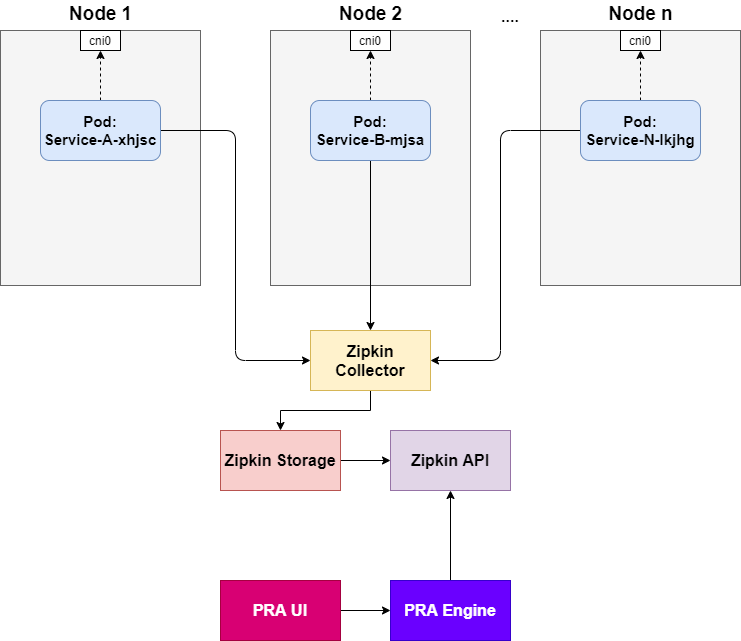
\includegraphics[width=1\textwidth]{resources/ch3/arch.png}
	\caption{Arsitektur sistem \textit{Performance Regression Analysis}}
	\label{arch-pra}
\end{figure}

\section{Jadwal Pelaksanaan}
 
 \newsavebox\mybox
 \begin{lrbox}{\mybox}
	     \begin{ganttchart}[
		     vgrid={*{6}{draw=none}, dotted},
		     x unit=.05cm,
		     y unit title=.6cm,
		     y unit chart=.6cm,
		     time slot format=isodate,
		     time slot format/start date=2016-09-01]{2021-09-01}{2022-04-30}
		     \ganttset{bar height=.6}
		     \gantttitlecalendar{year, month} \\
		     \ganttbar[bar/.append style={fill=blue}]{Studi Literatur}{2021-09-01}{2021-11-30}\\
		     \ganttbar[bar/.append style={fill=blue}]{Analisis Masalah}{2021-10-01}{2021-11-15}\\
		     \ganttbar[bar/.append style={fill=blue}]{Perancangan Solusi}{2021-11-01}{2021-12-15}\\
		     \ganttbar[bar/.append style={fill=blue}]{Implementasi}{2021-12-15}{2022-03-01}\\
		     \ganttbar[bar/.append style={fill=blue}]{Pengujian dan Analisis Hasil}{2022-02-01}{2022-04-30}
		     \end{ganttchart}
	 \end{lrbox}

 Pengerjaan tugas akhir ini direncanakan mulai pada September 2021 sampai April 2022. Pelaksanaan tugas akhir ini dibagi menjadi 5 tahap yang dapat dipetakan kepada metodologi pengerjaan sebagai berikut,
 \begin{enumerate}
	     \item Tahap 1: Studi Literatur
	     \item Tahap 2: Analisis Masalah
	     \item Tahap 3: Perancangan Solusi
	     \item Tahap 4: Implementasi
	     \item Tahap 5: Pengujian dan Analisis Hasil
	 \end{enumerate}
 
 Jadwal pelaksanaan tugas akhir berdasarkan metodologi pengerjaan tugas akhir dapat dilihat pada Tabel \ref{Gantt-Chart} dibawah ini.
 \begin{table}[htb]
	 \centering
	 \caption{Gantt Chart jadwal pelaksanaan tugas akhir}
	 \label{Gantt-Chart}
	 \tikz{
		   \node[inner sep=0pt,outer sep=0pt] (gantt)
		   {\begin{tabular}{c}
				     \toprule
				     \resizebox{\textwidth}{!}{\usebox\mybox} \\
				     \bottomrule
				    \end{tabular}%
			    };
		 }   
	 \end{table}



